%%%%%%%%%%%%%%%%%%%%%%%%%%%%%%%%%%%%%%%%%
% IISER Thiruvananthapuram Thesis Report Format
% LaTeX Template
%
% Author:
% Nikhil Alex Verghese, BS-MS 17
% PLEASE FORWARD ANY AND ALL SUGGESTIONS AND COMPLAINTS TO: nikhil.alexv@gmail.com
%
% READ ALL INSTRUCTIONS IN EACH TEX FILE CAREFULLY, ESPECIALLY THE MAIN REPORT FILE.
%
% License:
% CC BY-NC-SA 4.0 (http://creativecommons.org/licenses/by-nc-sa/4.0/)
%
%%%%%%%%%%%%%%%%%%%%%%%%%%%%%%%%%%%%%%%%%

%----------------------------------------------------------------------------------------
%	PACKAGES AND OTHER DOCUMENT CONFIGURATIONS
%----------------------------------------------------------------------------------------

\documentclass[12pt,a4wide]{report} % Set the font size (10pt, 11pt and 12pt) and paper size (letterpaper, a4paper, etc)

\usepackage[spanish]{babel}

%\usepackage[brazilian]{babel}
\usepackage[natbibapa]{apacite}
\bibliographystyle{apacite}




\usepackage{amsthm,amssymb,mathrsfs,setspace,pstricks,booktabs,mathtools,amsmath,geometry}

\usepackage{url}

% UNCOMMENT REQUIRED PACKAGES
%
% latexsym package contains few extra symbols.
% footmisc package for typesetting footnotes better.
% hypperref package for creating for reliable hyperlinks and customizations.
% tikz package for drawing graphs and diagrams (XY-pic is now outdated).
% xcolor package for better control over colours.
% biblatex package for bibliography-related (modern form of bibtex; biber and natbib also available, use only one).
% READ ALL ASSOCIATED PACKAGE HELP FILES CAREFULLY BEFORE USE.
%
% \usepackage{latexsym,footmisc,biblatex,hyperref,xcolor,tikz}.

%\usepackage{play}
\usepackage{epsfig}
%\usepackage[position=t,singlelinecheck=off]{subfig}
\usepackage{appendix}
\usepackage{longtable}
%\usepackage{natbib}
\usepackage{caption}
\usepackage{subcaption}
\usepackage{float}
\usepackage{multicol}
\usepackage{supertabular}
\usepackage{booktabs} % For better table rules
\usepackage{lipsum}
 \usepackage{epigraph}





%\usepackage[grey,times]{quotchap}
\usepackage[nottoc]{tocbibind}
\renewcommand{\chaptermark}[1]{\markboth{#1}{}}
\renewcommand{\sectionmark}[1]{\markright{\thesection\ #1}}

\setlength{\parskip}{1em plus 0.25em minus 0.25em}

\theoremstyle{plain}
\newtheorem{theorem}{Theorem}[section]
\newtheorem{lemma}[theorem]{Lemma}
\newtheorem{corollary}[theorem]{Corollary}
\newtheorem{proposition}[theorem]{Proposition}

\theoremstyle{definition}
\newtheorem{definition}[theorem]{Definition}
\newtheorem{example}[theorem]{Example}
\newtheorem{notation}[theorem]{Notation}

\theoremstyle{remark}
\newtheorem{remark}[theorem]{Remark}

\renewcommand{\baselinestretch}{1.5}
\newcommand{\RT}{RoBERTuito }
\newcommand{\BT}{BERTIN }
\newcommand{\BTO}{BETO }
\newcommand{\EL}{ELECTRICIDAD }
\newcommand{\BTA}{RoBERTa }
\newcommand{\TXL}{twitter-XLM }


% Uncomment below for headers and footers.
% Further customization codes can be referred here: https://www.overleaf.com/learn/latex/Headers_and_footers
%\usepackage{fancyhdr}
%\pagestyle{fancy}

% Uncomment for some standard notations in math (Real, Complex and Rational numbers, Norm, Jacobian, etc) %
%\newcommand{\reals}{\mathbb{R}}
%\newcommand{\complex}{\mathbb{C}}
%\newcommand{\rational}{\mathbb{Q}}
%\newcommand{\jacobian}{\mathcal{J}}
%\newcommand{\norm}[1]{\left\lVert #1 \right\rVert}

\begin{document}
\renewcommand{\BOthers}[1]{et al.\hbox{}}

% CUSTOM INPUT FIELDS ARE MARKED WITH [] IN THE INTRO SECTIONS.
% GO THROUGH EACH INTRO PAGE AND UPDATE ALL YOUR PERSONAL INFORMATION ACCORDINGLY.
% ALSO READ ALL UNCOMMENTED LINES CAREFULLY.

% --------------- Title page -----------------------%
\begin{titlepage}
\enlargethispage{3cm}

\begin{center}

\vspace*{-1cm}

\textbf{\Large Aplicación de modelos de lenguaje para la identificación de emociones en Twitter durante las elecciones presidenciales de 2022 en Colombia}\\[10pt]

\vspace*{0.5cm}


Tesis presentada para optar por el titulo de\\ 
\vspace*{0.5cm}
{\Large \bf Magister en Explotación de Datos y Descubrimiento del Conocimiento } \\





                      \vspace{10mm}
                   {\em  por} \\ \vspace{3mm}
             {\large \bf Juan Jose Iguaran Fernandez} \\


\vspace*{10mm}

\begin{figure}[h]
  \begin{center}
  \subfloat{{
\includegraphics[scale=0.55]{Images & Logos/data_mining.png} }}%
  \subfloat{{
\includegraphics[scale=0.18]{Images & Logos/uba.png}
   }}
  %
  \end{center}
\end{figure}

\vspace*{10mm}


{\bf\large Universidad de Buenos Aires} \\[10pt]
{\bf\large Facultad de Ciencias Exactas y Naturales}\\%[4pt]



{\bf\large Departamento de Ciencias de la Computación}\\%[8pt]
{\it\large [Insert Month and Year]}

\end{center}

\end{titlepage}

\clearpage



% Switch from 03a_Certificate (line 81) to 03b_Certificate (line 84) for a fancier format.
% You can disable geometry package if not switching and compile time is too long. 
% \thispagestyle{plain}
\newgeometry{left=1cm,top=2cm,right=1cm}


 \flushleft
 
\includegraphics[width=40mm]{Images & Logos/iiser_logo.png}

\vspace{0.5\baselineskip}
\hrule
\vspace{3\baselineskip}

\begin{center}
{\Large {\bf Certificate}}
\end{center}

\vspace{\baselineskip}

\noindent This is to certify that the work contained in this project report entitled
"\textbf{[Insert Project Title]}" submitted by \textbf{[Insert Name]} (Roll No. \textbf{[Insert Roll Number]}) to the Indian Institute of Science Education and Research, Thiruvananthapuram towards the partial requirement of {\bf [Master of Science/ Doctor of Philosophy]} in \textbf{[Branch of Science]} has been carried out by [him/her/them] under my supervision and that it has not been submitted elsewhere for the award of any degree.

\vspace{3\baselineskip}
\begin{flushright}
\begin{minipage}[c]{0.45\textwidth}
\centering
\vspace{3\baselineskip}
\hrule
\vspace{1.5\baselineskip}
{\large [Project Supervisor Name]} \bigskip\\
{\large \bf Project Supervisor} \\
\large [Insert Department] ~\\\
IISER Thiruvananthapuram
\end{minipage}
\end{flushright}
\vspace{\baselineskip}
\restoregeometry

% Credit for Certificate code file: Sagnik Saha, IISER B'16
% ----------------- Acknowledgement page--------------------%
\begin{center}
{\large{\bf{AGRADECIMIENTOS}}}
\end{center}
%\thispagestyle{empty}


\noindent
 Quiero agradecer a la Maestría por todo el conocimiento y la formación brindada sin los cuales cual este trabajo no habría sido posible. Agradezco también a mis directores por todo su apoyo, paciencia y mentoría a lo largo de este proceso.
 
 A Luis Felipe Nuñez, cuyas valiosa palabras  ''Tomate en serio'' forjaron mi motivación. A Jaime Diaz, gracias a quien pude iniciar este viaje y estuvo presente de muchas formas. A Carolina Franco cuyo afecto, apoyo y acompañamiento fueron claves durante este proceso, y a Judith Fernandez, la autora de mi vida.
 


\vspace{4cm} %Reduce if text overflowing to a new page



\clearpage
% ----------------- Acknowledgement page--------------------%
\begin{center}

\end{center}
%\thispagestyle{empty}



 
 \epigraph{Todos los estados encuentran su origen en la mente. La mente es su fundamento y son creaciones de la mente. 
 	Si uno habla o actúa con un pensamiento impuro, entonces el sufrimiento le sigue de la misma manera que la rueda sigue la pezuña del buey... 
 	
 	Todos los estados encuentran su origen en la mente. La mente es su fundamento y son creaciones de la mente. 
 	Si uno habla o actúa con un pensamiento puro, entonces la felicidad le sigue como una sombra que jamás le abandona. \par\hfill\textsc{---\textit{Dhammapada}}}

\vspace{4cm} %Reduce if text overflowing to a new page



\clearpage
% -------------------- Abstract page -----------------------%
\begin{center}
{\Large{\bf{Resumen}}}
\end{center}



Twitter ha sido analizado como un medio particularmente interesante para el estudio indirecto de fenómenos sociales a través del uso de técnicas del procesamiento del lenguaje natural (NLP) pues es capaz de captar a una gran cantidad de usuarios sobre una gran numero de tópicos en una cantidad limitada de palabras con estilo propio. Esto ha sido estudiado en el pasado en por ejemplo, como los análisis de texto provenientes de este, coincide con lo que arrojan otras aproximaciones de las realidades sociales tales como las encuestas de opinión, discursos políticos o eventos de relevancia popular. 

Una tarea en particular dentro del NLP,  la detección de emociones, resulta de particular interés al estudiar la respuesta individual a fenómenos sociales pues dentro del texto existe información objetiva, como hechos verificables e información subjetiva, que corresponde a los procesos internos que los individuos experimentan y son plasmados en el texto, tal como las opiniones. 
Las emociones son parte de esta información subjetiva, y su clasificación en términos generales ha sido definida en seis emociones básicas: miedo, rabia, tristeza, alegría, sorpresa y disgusto. En ese contexto, la detección de las emociones presentes en el texto es un sub campo del análisis de sentimiento en el texto que busca determinar la polaridad y el grado de las distintas dimensiones de la subjetividad presentes en el texto.


El estudio del análisis de sentimientos en general y de emociones en particular se ha hecho usualmente a través tradicionales de NLP tales como el empleo de modelos de aprendizaje supervisado a partir de features construidos a partir del texto.
Durante los últimos años, estas técnicas están siendo remplazadas por modelos de lenguajes usando redes neuronales, en particular arquitecturas como los Transformers debido a su capacidad de tener en cuenta el contexto dentro del cual se encuentran las palabras en el texto, es decir, su relación con otras palabras. Una aplicación particular de los Transformers BERT, es particularmente útil pues consiste en un modelo pre entrenado que es capaz de desempeñar la tarea de NLP en particular para la cual se haga un entrenamiento final

En español existen pocos casos de detección de emociones en redes sociales, y no se conoce de ninguno que use modelos de lenguaje basado en Transformers para este fin en un contexto político.
EL presente  trabajo tiene por objetivo el empleo de modelos de lenguaje, específicamente  BERT que es un una red neuronal pre entrenada con la wikipedia basada en Transformers para detectar emociones presentes en twitter durante las elecciones en Colombia.

\vspace{4cm} % Reduce if text overflowing to a new page. Don't make it too long.
\textbf{Palabras Clave:} [BERT, Colombia, Elecciones, Detección de emociones]

\clearpage
% ------------------ Table of Contents --------------------%

\tableofcontents
\clearpage
\listoffigures
\listoftables

\newpage

\pagenumbering{arabic}
\setcounter{page}{1}

% =========== Main chapters starts here =================== %

\chapter{Introduccion}


Twitter ha sido analizado como un medio particularmente interesante para el estudio indirecto de fenómenos sociales a través del uso de técnicas del procesamiento del lenguaje natural (NLP) pues es capaz de captar a una gran cantidad de usuarios, que discuten sobre una gran numero de tópicos, usando en una cantidad limitada de palabras con estilo propio. Esto ha sido estudiado en el pasado por ejemplo, al analizar como los textos provenientes de este medio, coinciden con lo que arrojan otras aproximaciones de las realidades sociales tales como las encuestas de opinión, discursos políticos o eventos de relevancia popular. 

Una tarea en particular dentro del NLP,  la detección de emociones, resulta de particular interés al estudiar la respuesta individual a fenómenos sociales, pues dentro del texto existe tanto información objetiva, que corresponde a hechos verificables, como información subjetiva, que corresponde a los procesos internos que los individuos experimentan y son plasmados en el texto, tal como las opiniones. 
Las emociones son parte de esta información subjetiva, y en ese contexto, la detección de las emociones presentes en el texto, se define como un sub campo del análisis de sentimiento, que busca determinar la polaridad y el grado de las distintas dimensiones de la subjetividad presentes en el texto.


El estudio del análisis de sentimientos en general y de emociones en particular, se ha hecho usualmente a través de técnicas tradicionales de NLP tales como el empleo de modelos de aprendizaje supervisado usando de features construidos a partir del texto.
Durante los últimos años, estas técnicas están siendo remplazadas por modelos de lenguajes usando redes neuronales, en particular arquitecturas como los Transformers, debido a su capacidad de tener en cuenta el contexto dentro del cual se encuentran las palabras en el texto, es decir, su relación con otras palabras. Una aplicación particular de los Transformers BERT, es particularmente útil pues consiste en un modelo pre entrenado que es capaz de desempeñar la tarea de NLP particular, para la cual se haga un entrenamiento final.

En español existen pocos estudios de detección de emociones en redes sociales, y no se conoce de ninguno que use modelos de lenguaje basado en Transformers para este fin en un contexto político.
EL presente  trabajo tiene por objetivo el empleo de modelos de lenguaje, específicamente  BERT que es un una red neuronal pre entrenada con la Wikipedia basada en Transformers para detectar emociones presentes en twitter durante las elecciones presidenciales en Colombia en 2022. 

Para poder obtener los datos de entrenamiento, se hará uso de una base de datos obtenida mediante la descarga tweets, a través de la API, utilizando hashtags relacionados al tema de las elecciones, entre el 22 de mayo y el 22 de junio del 2022, periodo que contiene la primera y segunda vuelta presidencial de las elecciones en Colombia. Estos hashtags, y por consiguiente los tweets relacionados a estos, serán asociados por el autor a los sectores políticos izquierda, derecha o neutro, basándose en el contenido observado en los tweets y el apoyo o rechazo que estos muestren. A partir de ahí, se procederá a tomar una muestra de 1200 tweets para ser etiquetados manualmente por el autor y los directores, en alguna de las emociones disponibles. Con los tweets etiquetados, se procederá a realizar el fine tuning de varios modelo de lenguaje pre entrenados y evaluar su desempeño para escoger el mejor. Este modelo, sera utilizado para clasificar toda la base de datos y a partir de esta clasificación,  realizar agrupaciones que permitan determinar la respuesta emocional de los tweets asociados a cierto sector político, así como la variación temporal de esta respuesta. 



\chapter{Introducción}






\section{Motivación}

Este trabajo es importante por que 



\section{Marco Teórico}

En \cite{ekman1993facial} Ekman realiza un estudio de la respuesta fisiológica en general y de las  expresiones faciales del ser humano en diferentes culturas ante distintas circunstancias. Esto lo lleva a concluir que existen grandes grupos en donde las distintas expresiones faciales pueden ser agrupadas ya que estas reflejan el estado emocional interno de los individuos. A estos grupos los denomino emociones básicas y son los siguientes: Alegría, enojo, sorpresa, asco, miedo y tristeza. Este modelo de emociones básicas es comúnmente usado para los estudios relacionados con las emociones.

En el libro \cite{picard2000affective} Picard expone su punto de vista en donde parte de recientes investigaciones en psicología cognitiva que exponen las emociones como un componente fundamental de la inteligencia humana, por lo que la· búsqueda de una inteligencia artificial capaz de interactuar eficazmente con los seres humanos, debe traer consigo la capacidad de reconocer, entender, tener y expresar emociones. A partir de ahí expone los avances hechos hasta la fecha en el terreno de lo que ella llama, computación afectiva.

En \cite{ortony1987referential} se habla de como a pesar de que las emociones son procesos mentales internos que no residen en el lenguaje, este es el medio no fenomenológico mas conveniente a través del cual podemos acceder a ellas. Elabora entonces una serie condiciones que deben estar presentes en los términos para poder referirse de una manera acertada a los estados emocionales, y las aplica sobre términos presentes en la literatura con respecto a las emociones, construyendo así un léxico emocional.


En \cite{hatzivassiloglou1997predicting} a partir de un corpus extenso de adjetivos que vienen en parejas con usando distintos conectores, y un etiquetado manual de algunos de ellos, se establece un algoritmo para determinar lo que los autores denominan la orientación semántica de los mismos, esto es determinar si determinado adjetivo tiene una connotación negativa o positiva de la característica que describe. Este método permite la creación automática de un corpus extenso de adjetivos cuyo sentimiento se encuentra identificado.

En \cite{strapparava2004wordnet} se realiza una anotación manual de estados emocionales basados en las categorías de \cite{ortony1987referential} sobre algunos términos encontrados en WordNet \cite{miller1995wordnet}, que es una base de datos de términos en ingles agrupados por grupos de sinónimos y con relación semántica entre grupos. A partir de ahí se establece la categoría emocional de nuevos términos gracias a los sinónimos y las relaciones semánticas, construyendo así una base de datos de estados emocionales llamada WordNet-Affect

En \cite{wiebe1994tracking} se pone de manifiesto que en un tipo particular de texto, la ficción, la narración puede ocurrir desde un punto de vista objetivo,m es decir, una descripción de hechos comprobables, y también desde un punto de vista subjetivo, es decir, poniendo de manifiesto los hechos atravesados por los estados mentales internos el narrador, y que la distinción entre un tipo de narración y otra no esta siempre clara, por lo que propone un algoritmo capaz de hacer esta distinción de manera automática.


En \cite{yu2003towards} se plantea la necesidad de sistemas algoritmos capaces de discernir opiniones de hechos con el objetivo de lograr sistemas capaces de responde preguntas. Esta necesidad se plante a nivel de documentos, por ejemplo diferenciar editoriales de artículos de noticias, así como a nivel de frases. se plantean distintos modelos de aprendizaje supervisado para estas tareas en particular.



En \cite{pang2002thumbs} se establece la importancia de desarrollar, ante textos que reflejen opiniones subjetivas, sistemas capaces de identificar si dicha opinión es negativa o positiva. Para este propósito, se emplea el dominio de las reviews online de películas, construyendo algoritmos de aprendizaje supervisado que utiliza como features principalmente unigramas.

En \cite{turney2002thumbs} se pretende determinar a traves de aprendizaje no supervisado, si determinada review sobre diversos temas online, presenta un sentimiento negativo o positivo. Para ello, emplea el concepto de orientación semántica presente en \cite{hatzivassiloglou1997predicting} para determinar si una frase tiene orientación negativa o positiva para luego determinar si la review en su conjunto es positiva o negativa.

En \cite{wiebe2005annotating} se elabora una anotación manual de las estados emocionales presentes en las oraciones de un gran volumen de noticias, en donde se tiene en cuenta el contexto. El objetivo de esta anotación es crear un corpus etiquetado lo suficientemente grande para generar avances en el campo de la detección de emociones

En \cite{alm2005emotions} se utilizan los cuentos infantiles para desarrollar un modelo de aprendizaje supervisado capaz de detectar emociones en las frases del texto. Para ello se elabora una anotación manual de las frases que constituyen el set de datos y luego, se generan un set de features para estas que pasaran a entrenar un clasificador lineal.

En \cite{aman2007identifying} se utilizan texto proveniente de blogs para realizar detección de emociones presentes en las oraciones de estos. Para ello recurren primero a una anotación manual de las mismas y luego a la construcción de features para entrenar distintos modelos supervisados.


Luego, en \cite{pang2008opinion} se hace manifiesto la importancia que ha venido ganando el campo del análisis de sentimiento debido al auge del Internet, tanto para usuarios individuales como para la industria de la publicidad, el mercado financiero y la academia, por lo que se hace un recuento de las distintas técnicas y aplicaciones que son consideradas relevantes por los autores hasta la fecha. 




En \cite{pak2010twitter} se identifica twitter como una plataforma útil para extraer texto de diferentes usuarios sobre distintos temas por lo que se propone realizar un análisis de sentimientos sobre la misma. Para ello se procede  a la identificación de tweets que contengan emoticones felices y tristes, así como tweets provenientes de cuentas de medios de noticias para tweets neutrales. luego se procede a la construcción de features usando n-gramas a partir de las palabras presentes en el tweets  con estos se entrenaron varios clasificadores.



En \cite{o2010tweets} se plantea la pregunta si existe una correlación entre el sentimiento encontrado en twitter y las encuestas de opinión. Para ello, se toma una muestra del de mil millones de tweets entre 2008 y 2009 y se toman aquellos tweets que contengan palabras claves asociadas a los temas que se están investigando. EL sentimiento se determina a partir de la proporción de palabras con asociación negativa o positiva presentes en el tema que se esta analizando en un día en particular. Los resultados dan una correlación alta entre el sentimiento encontrado a través del texto y las encuestas.

En \cite{davidov2010enhanced} se parte del supuesto de que los hashtags y los emoticones contienen información relevante el cuanto al sentimiento del tweet, por lo que se hace una selección de 50 hashtags que tengan una asociación fuerte al sentimiento y se entrena un modelo supervisado a partir de los tweets que contengan estos hashtags, construyendo un vector de features para cada uno. El modelo es posteriormente empleado para clasificar otros tweets y jueces humanos verifican su eficacia.


En  \cite{wang2012harnessing} se entrena un modelo de supervisado distante de emociones presentes en twitter. Para ellos, se utilizan hashtags que contengan terminos claves provenientes de las 5 emociones basicas de propuestas por \cite{ekman1993facial} para realizar el llamado de la api. A partir de ahi se entrena el modelo a partir de los features construidos para el texto de los tweets. 

En \cite{roberts2012empatweet} se identifica la necesidad de contar con un corpus que sirva de base para la tarea de identificación de emociones en twitter. Para ello, se seleccionan  14 temas que para los autores tienen un fuerte contenido emocional y las palabras clave asociados a estos para ser usados como hashtags en las extracción. A partir de ahí, manualmente se etiquetaron los tweets con su respectiva emoción. Esto sirvió de base para entrenar un modelo de aprendizaje supervisado.



En \cite{bollen2011modeling} se plantea que a través del uso de twitter, los usurarios reflejan sus estados emocionales, ya sea de una manera explicita al indicar su emoción o de una manera implícita al hablar sobre un tema de interés general. En ese contexto, se genera procede a realizar una medida del estado emocional de una muestra de tweets entre agosto y diciembre del 2008, en donde el mismo se mide a través de ka similaridad presente entre las palabras de los tweets y ciertos términos claves asociados a estados emocionales. Esto permite encontrar que determinados eventos relevantes generan un impacto emocional significativo y durante un periodo de tiempo en los usuarios.

En \cite{tumasjan2010predicting} se plante el uso de twitter como plataforma de medición de la sensación política durante las elecciones parlamentarias en Alemania en el 2009. Una de sus preguntas de investigación estuvo relacionada con los sentimientos que se reflejan en los tweets que mencionan a los políticos que hacen parte de las campañas y para esto, se empleo sobre el texto proveniente de twitter, un software capaz de identificar palabras claves asociadas a estados emocionales y cognitivos en el texto. El resultado fue un perfil emocional para cada político que ve de acuerdo con su discurso político.

En \cite{ceron2016sentiment} se pretende realizar un análisis de sentimientos sobre tweets relacionados con las elecciones presidenciales en Colombia en el 2014 y comparar los resultados de este con las encuestas de opinión. Para ellos, inicialmente obtiene tweets que tengan  palabras claves y hashtags relacionados con las elecciones, luego hace un filtrado de spam y finalmente entrena un modelo supervisado con los features que genera para los tweets restantes. Los resultados no son consistentes por lo que se plantea en futuros trabajos  una caracterización demográfica.



Las RNN (redes neuronales recurrentes) son un tipo de arquitectura de red neuronal cuyo uso es especial para datos secuenciales, tales como las tareas de NLP. En estas, para un ejemplo nuevo, es posible utilizar el resultado del procesamiento de un dato anterior, para el procesamiento del siguiente dato (como en una secuencia de caracteres por ejemplo), es decir la misma topología de pesos recibirá para cada ejemplo nuevo, el resultado del ejemplo anterior ademas del ejemplo nuevo de entrada. Sin embargo, debido a su arquitectura, la optimizacion de los pesos que constituyen la topología se vuelve compleja pues para el calculo del gradiente del error, se deberá pasar tantas veces por los pesos de la red como pasos en el tiempo haya (como numero de caracteres en una palabra) haciendo que en secuencias particularmente largas, este calculo crezca o disminuya en demasía. Para enfrentar este problema , \cite{hochreiter1997long} y \cite{chung2014empirical} plantean nuevas arquitecturas de RNN conocidas como LSTM (Long-Short term memoryzz) y GRU (Gated Recurrent Unit) respectivamente, en donde a través de nuevas unidades que permiten la activación/cancelación de las señales que constituyen la red, se puede realizar la optimizacion de manera directa sin pasar por los pesos de la red.


En general ,las arquitecturas de RNN, al tener una estructura secuencial, se impide la paralelizacion de su computo, pues se necesita las salidas de ejemplos anteriores para llevar a cabo el siguiente paso en el tiempo. Ademas, debido a esta mismo funcionamiento secuencial, si existe un gran numero de pasos en el tiempo, es poco probable que la red tenga en cuenta información presente al inicio. Para solucionar estos inconvenientes, \cite{vaswani2017attention} desarrollan los Transformers, que son un tipo de arquitectura en la que todos los datos de entrada, son ingresados a la red de manera simultanea, como todas las palabras en una frase por ejemplo, y a través de una arquitectura que definen como atención, se realiza una transformación de los datos de manera que la representación de cada dato, en este caso cada palabra, tenga en cuenta que tan importante es la misma para todas las demás palabras de la oración. Esta transformación, aplicada tanto en los datos de entrada como en los de salida, es luego usada para entrenar los pesos de la red. De esta manera la red es capaz de procesar datos en simultaneo así como tener en cuenta toda la información disponible.
 

En \cite{devlin2018bert} se desarrolla BERT

En \cite{acheampong2021transformer} se hace un recuento de el uso de transformers para detectar emociones

EN \cite{canete2020spanish} se propone una aplicación de BERT para español

En \cite{gonzalez2021twilbert}, \cite{huang2019ana} se utiliza bert en twitter para  detectar emociones

En \cite{plaza2020improved}, \cite{gil2013combining} se hace una clasificación de emociones en español.


En \cite{sidorov2012empirical} propone un léxico de palabras en español asociadas a emociones
`









\chapter{Metodología}


\chapter{Resultados}



En el gráfico \ref{figure:Entrenamiento_modelos} se puede observar los resultados de la metrica micro F1 para los distintos modelos escogidos, a lo largo de su entrenamiento. Cabe resaltar que son los resultados promedio de cada modelo estos se entrenaron 10 veces cada uno cambiando su semilla. Se observa entonces que el de mejor comportamiento fue el robertuito-base-uncased con un micro f1 al final de su entrenamiento de 0.8393, siendo asi el modelo escogido.


\begin{figure}[h]
	\caption{Entrenamiento de los modelos}
	\centering
	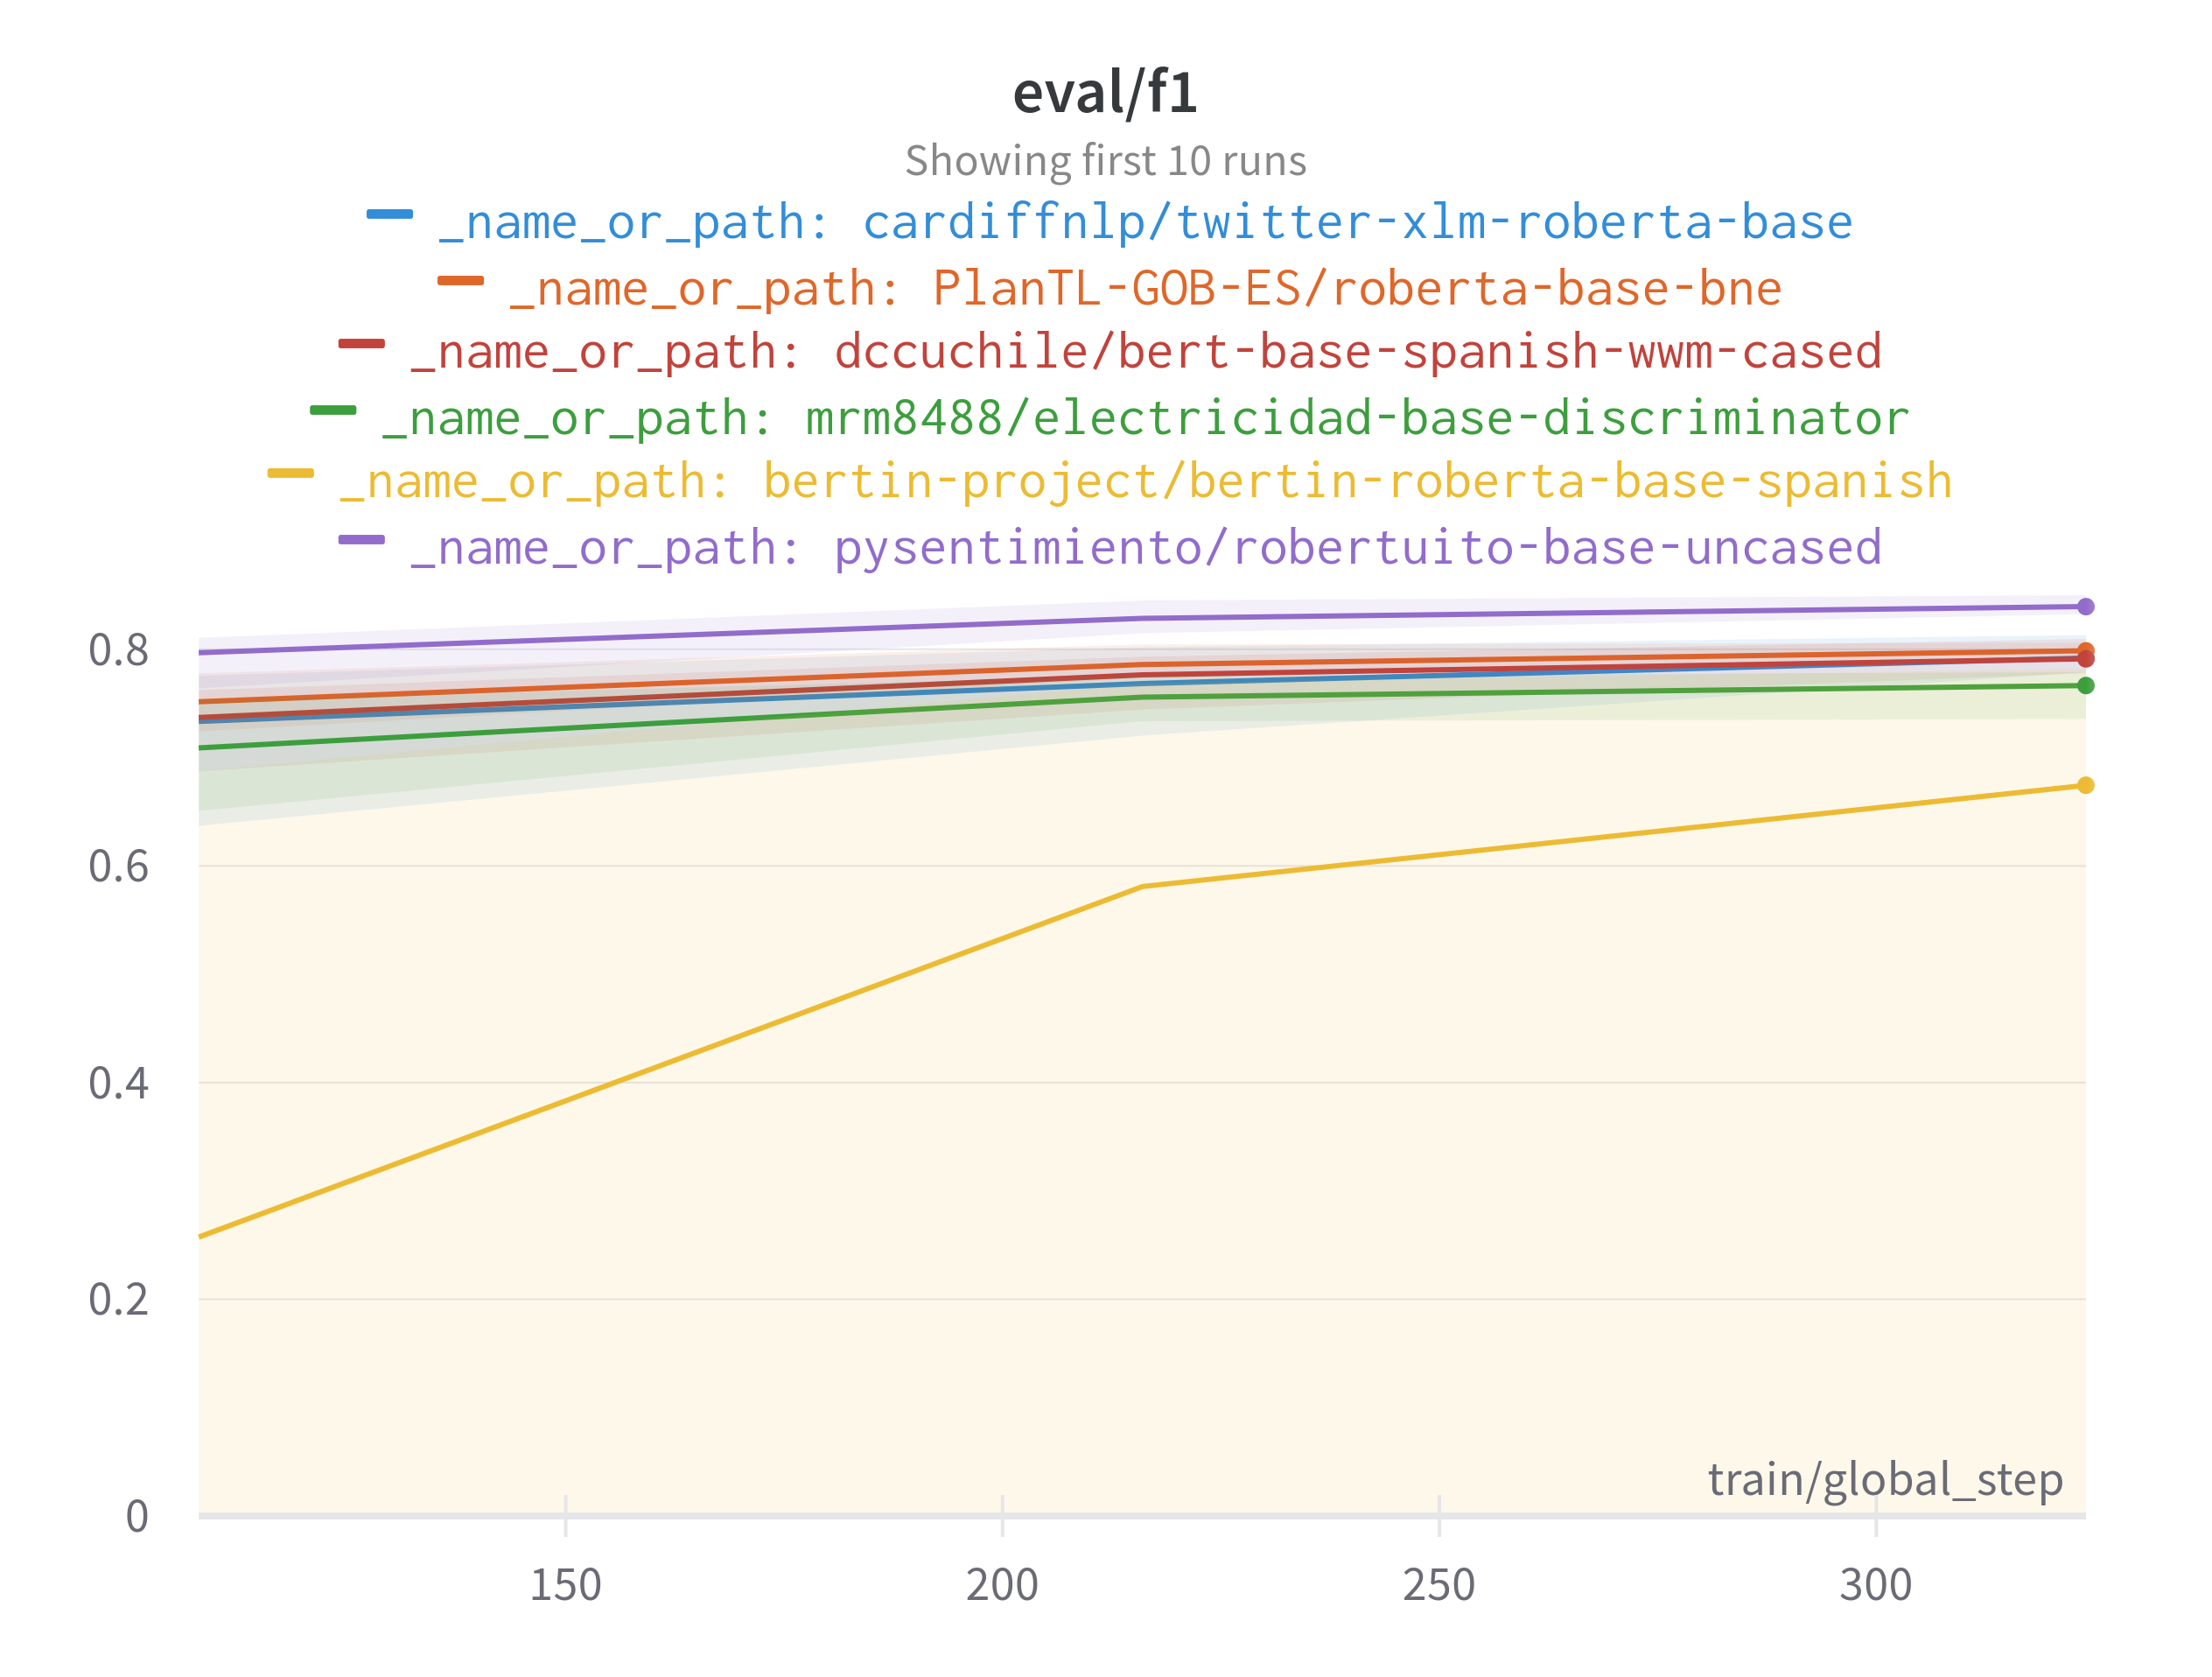
\includegraphics[scale=0.15]{../Images/Results/W&B Chart 5_18_2023, 7_25_13 PM (1).png} 
	\label{figure:Entrenamiento_modelos}
\end{figure}


\section{Distribución de emociones por sector}

Una vez desplegado el modelo y obtenido las etiquetas emocionales para todos los tweets del dataset se obtienen los resultados obtenidos en el gráfico \ref{figure:tweets_total}, en donde se aprecia el porcentaje de tweets que recibió cada una de las distintas etiquetas. Allí puede apreciarse que la emoción mas preponderante fue el asco, con mas del 50\% de los tweets. Luego fue la alegría, con alrededor del  40\%. Finalmente, el miedo y la tristeza estuvieron mucho menos presentes con menos del 3\% cada una. 

\begin{figure}[h]
	\caption{Porcentaje de tweets por emociones}
	\centering
	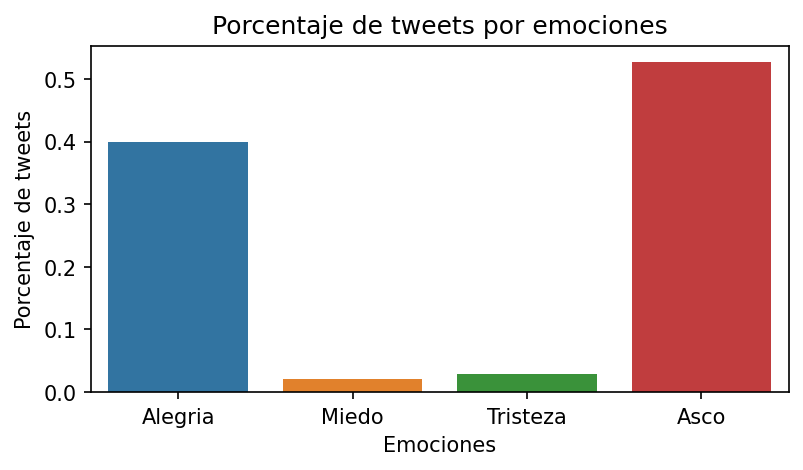
\includegraphics{../Images/Results/Cantidad_de_tweets__por_emocion.png} 
	\label{figure:tweets_total}
\end{figure}



Al analizar la presencia emocional de cada emoción en los distintos sectores políticos, se obtuvieron los resultados que se presentan en el gráfico \ref{figure:tweets_percent_miedo}. En dicho gráfico se observa que el sector neutral fue el que mostró una mayor cantidad de tweets etiquetados con miedo, representando aproximadamente el 3\% de sus tweets. En cambio, tanto la izquierda como la derecha tuvieron una presencia menor, con alrededor del 1.2\% y 0.8\% respectivamente.








\begin{figure}[h]
	\caption{Porcentaje de tweets por sector etiquetados con Miedo}
	\centering
	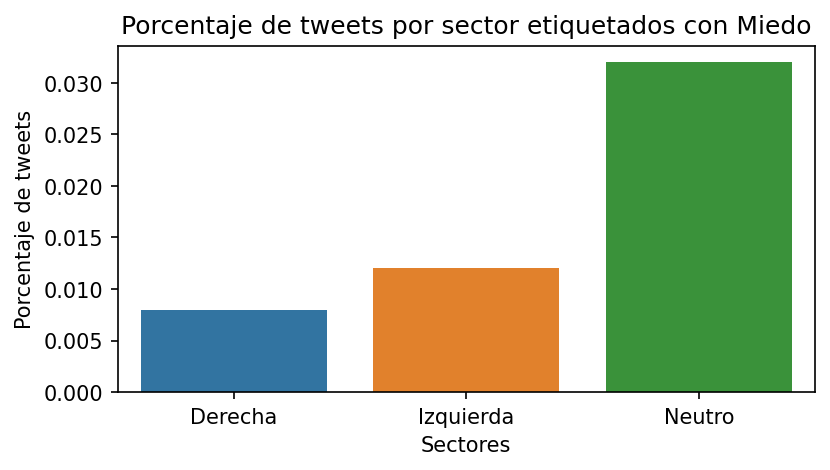
\includegraphics{../Images/Results/Porcentaje de tweets por sector etiquetados con Miedo.png} 
	\label{figure:tweets_percent_miedo}
\end{figure}

En relación a la emoción de alegría, el gráfico \ref{figure:tweets_percent_alegria} revela que la izquierda fue el sector que mostró una mayor presencia de dicha emoción en sus tweets, alcanzando el 55\%. En segundo lugar se encuentra el sector neutral, con un 33\%, seguido por la derecha con un 29\%.

\begin{figure}[h]
	\caption{Porcentaje de tweets por sector etiquetados con Alegría}
	\centering
	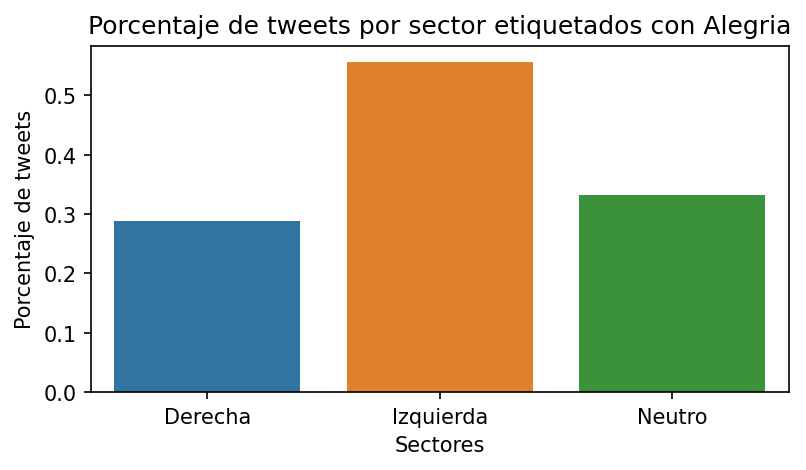
\includegraphics{../Images/Results/Porcentaje de tweets por sector etiquetados con Alegria.png} 
	\label{figure:tweets_percent_alegria}
\end{figure}

En cuanto al asco, se destaca la participación predominante de la derecha, como se observa en el gráfico \ref{figure:tweets_percent_asco}, representando un 69\% del total de sus tweets. El sector neutral se posiciona en segundo lugar con un 54\% de los tweets, dejando a la izquierda con el menor porcentaje de los tres, un 40\%.

\begin{figure}[h]
	\caption{Porcentaje de tweets por sector etiquetados con Asco}
	\centering
	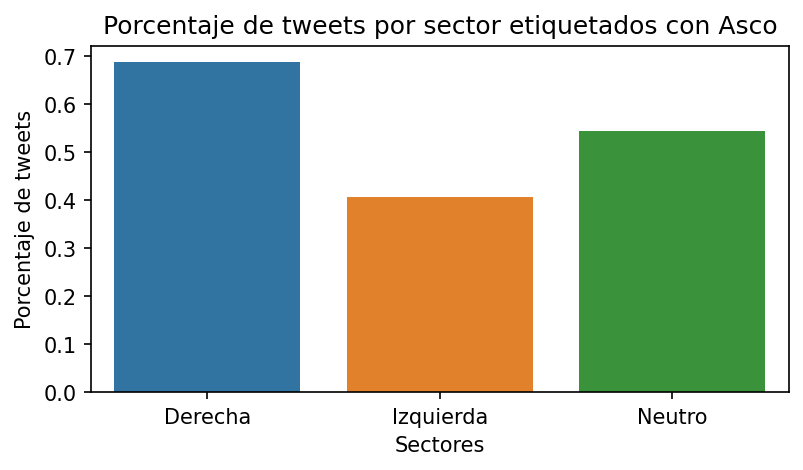
\includegraphics{../Images/Results/Porcentaje de tweets por sector etiquetados con Asco.png} 
	\label{figure:tweets_percent_asco}
\end{figure}


Finalmente, para la tristeza, el sector neutro fue en donde esta emocion tuvo mayor presencia con un 5\% de su total, lo cual fue bastante mayor que la izquierda y la derecha, con un un .08 y .04\% respectivamente.

\begin{figure}[h]
	\caption{Porcentaje de tweets por sector etiquetados con Tristeza}
	\centering
	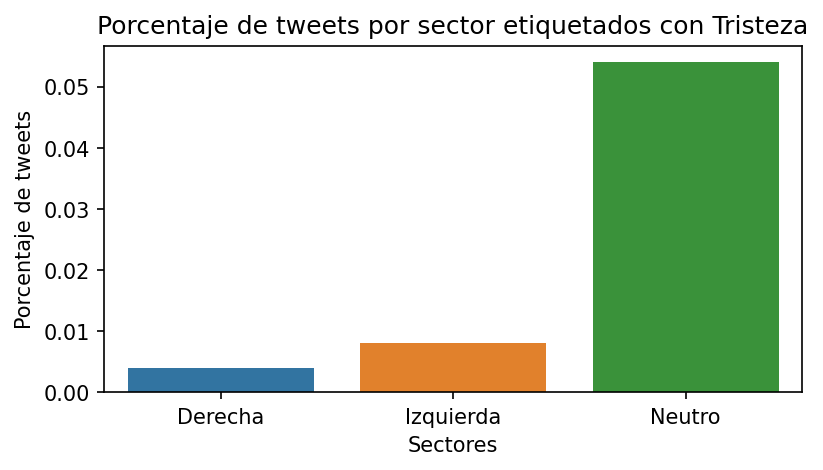
\includegraphics{../Images/Results/Porcentaje de tweets por sector etiquetados con Tristeza.png} 
	\label{figure:tweets_percent_tristeza}
\end{figure}




\section{Emociones a lo largo del tiempo}


Para determinar para cada emoción, que porcentaje de esta etiqueta tuvo un día en particular, se  dividió el numero tweets con esta emoción en dicho día sobre el total de tweets con esta etiqueta. De esta manera, se aprecia en el gráfico  \ref{figure:tweets_percent_tiempo}, que el 29 de mayo fue particularmente activo pues contó con casi 40\% de los tweets con miedo, y un 26\% de los tweets con alegría y tristeza. Este fue el día de la primera vuelta presidencial. Del mismo modo, se aprecia como los días 9 y 10 de junio tuvieron un repunte de asco y tristeza respectivamente, con un 9 y 11\%. Estos días estuvieron marcados con el evento de los llamados Petro videos. Luego hay un repunte de asco y tristeza al rededor del 16 de junio, fecha en donde se hablo del debate final al cual Rodolfo Hernandez se negó a participar, y finalmente de alegría, tristeza y miedo para el 19 de junio que fue la segunda vuelta.

\begin{figure}[h]
	\caption{Porcentaje de tweets por sector etiquetados con Tristeza}
	\centering
	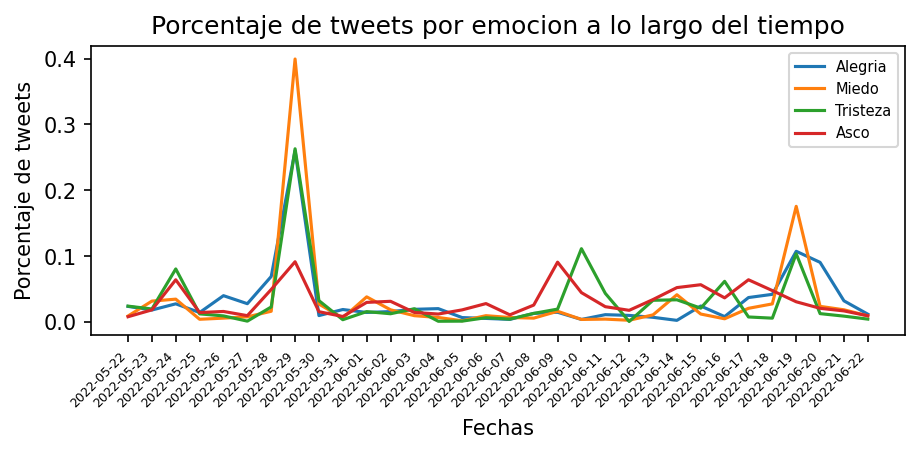
\includegraphics{../Images/Results/Porcentaje de tweets por emocion a lo largo del tiempo.png} 
	\label{figure:tweets_percent_tiempo}
\end{figure}



Para cada emoción y cada sector, se obtuvo que porcentaje de esta etiqueta tuvo este sector un día en particular, al dividir el numero de tweets que este sector tuvo con esta etiqueta en dicho día sobre el total de tweets que este sector tuvo con esta etiqueta. De esta manera, se obtiene el gráfico \ref{figure:tweets_percent_alegria_tiempo} en donde se aprecia que el 29 de mayo todos los sectores tuvieron un repunte. Luego los tres sectores van creciendo cercanos al 19 de junio, para decaer eventualmente primero la derecha, luego el sector neutro y finalmente la izquierda.




\begin{figure}[h]
	\caption{Porcentaje de tweets con Alegría por sector lo largo del tiempo}
	\centering
	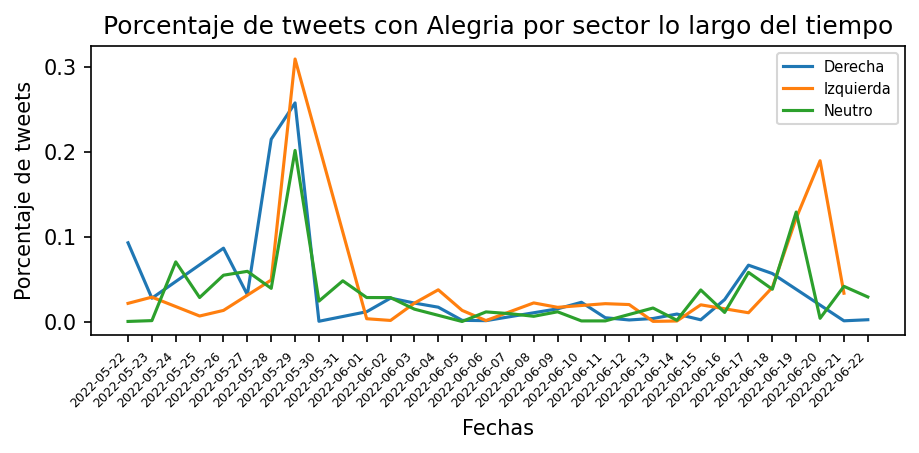
\includegraphics{../Images/Results/Porcentaje de tweets con Alegria por sector lo largo del tiempo.png} 
	\label{figure:tweets_percent_alegria_tiempo}
\end{figure}


Para el caso del miedo, se observa un gran pico de los tres sectores el 29 de mayo. Luego, para el 14 de junio, hubo un pico de miedo en la derecha como consecuencia a los rumores de estallido social, para finalmente haber un pico de miedo del sector neutro y de la izquierda cercano al 19 de junio.

\begin{figure}[h]
	\caption{Porcentaje de tweets con Miedo por sector lo largo del tiempo}
	\centering
	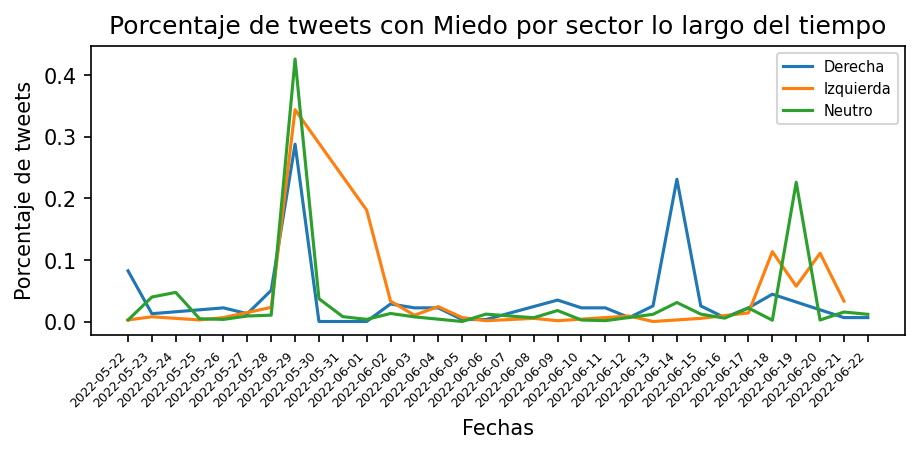
\includegraphics{../Images/Results/Porcentaje de tweets con Miedo por sector lo largo del tiempo.png} 
	\label{figure:tweets_percent_Miedo_tiempo}
\end{figure}


En cuanto a la tristeza, se aprecia que los tres sectores tuvieron un repunte el 29 de mayo, principalmente la izquierda en donde este dia se llego a casi un 40\%. Luego el 9 de junio hubo un repunte en la derecha, ligado al evento de los petro videos, y luego el 10 un repunte del sector neutro en donde se discutieron temáticas decepcionantes de las elecciones. Para el 14 de junio, la derecha tuvo devuelta un repunte de tristeza ligado, al igual que para el miedo, a la temática del estallido social. Finalmente, los tres sectores tuvieron un incremento de la tristeza para el 19 de junio.

\begin{figure}[h]
	\caption{Porcentaje de tweets con Tristeza por sector lo largo del tiempo}
	\centering
	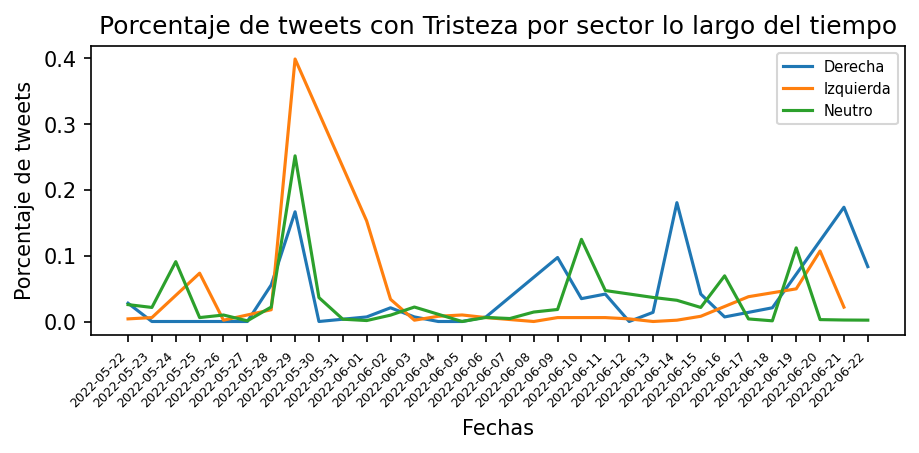
\includegraphics{../Images/Results/Porcentaje de tweets con Tristeza por sector lo largo del tiempo.png} 
	\label{figure:tweets_percent_Tristeza_tiempo}
\end{figure}

En cuanto al asco, al inicio hay un pico del sector neutro el 24 de mayo debido a las reacciones respecto a n debate. Luego, hubo un repunte de los tres sectores para el 29 de mayo. Se destaca el gran pico que tuvo la derecha, con mas del 25\%. Asi mismo, se observa que la izquierda tuvo su pico el 17 de junio con cerca del 20\%. En esta fecha fue en donde se hablo de la negativa de Rodolfo Hernandez a participar en el debate final

\begin{figure}[h]
	\caption{Porcentaje de tweets con Asco por sector lo largo del tiempo}
	\centering
	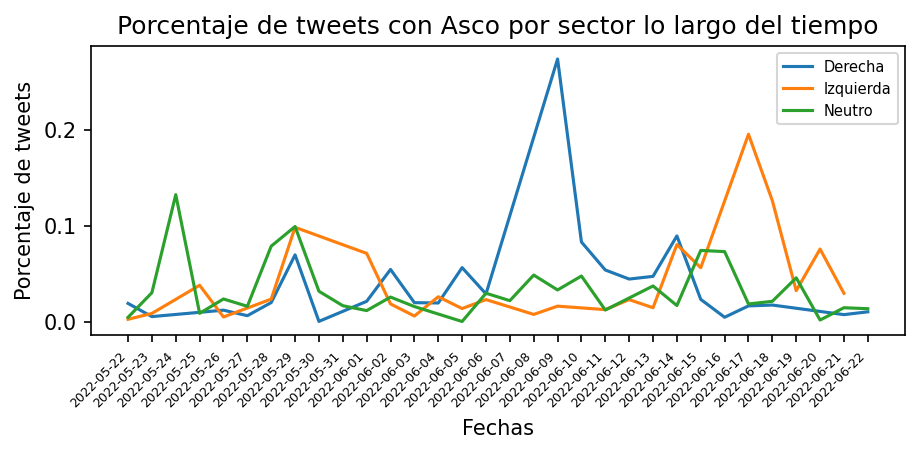
\includegraphics{../Images/Results/Porcentaje de tweets con Asco por sector lo largo del tiempo.png} 
	\label{figure:tweets_percent_Asco_tiempo}
\end{figure}















\chapter{Conclusiones}
 

El presente trabajo logró, a través del fine tuning de un modelo de lenguaje preentrenado, en este caso "robertuito-base-uncased", identificar las emociones presentes en los tweets relacionados con las elecciones presidenciales en Colombia del 2022. Estas predicciones permitieron poder asociar estas emociones a distintas orientaciones políticas, a partir de la asignación de una orientación a un tweet en particular, a partir del hashtag usado y la tendencia observada en el mismo. Así mismo , se pudo observar la fluctuación por emoción y por sector de los tweets a lo largo del periodo estudiado.

El proceso de fine tuning fue posible gracias a la creación de un recurso propio, un conjunto de datos de 1200 tweets etiquetados manualmente por el autor y los directores. Esta tarea de etiquetado se realizó utilizando una interfaz web y siguiendo un manual interno que permitió asignar una o varias de las 14 emociones disponibles a cada tweet. Para que una emoción fuera asignada al tweet, al menos dos etiquetadores debían coincidir en ella. Finalmente, cada tweet se clasificó con una de las cuatro etiquetas resultantes de la agrupación de las etiquetas originales, basada en su correlación. Es importante señalar la dificultad inherente en la tarea de etiquetado, ya que intenta lograr una clasificación objetiva de una actividad subjetiva, lo que requirió un proceso iterativo para desarrollar un manual y una interfaz de etiquetado que se acercara a este propósito. Además, aunque todos los etiquetadores son hispanohablantes nativos, solo el autor es originario de Colombia, lo que llevó a que ciertos usos del lenguaje o situaciones contextuales específicas fueran más claros para él que para los otros etiquetadores.

Las agregaciones de las predicciones realizadas por el modelo coinciden con las respuestas emocionales esperadas en ciertos eventos importantes durante las elecciones. Los resultados del modelo muestran una presencia mucho mayor de alegría y asco que de miedo y tristeza, lo cual concuerda con lo observado durante el proceso de etiquetado, ya que estas dos emociones fueron menos frecuentes y a menudo acompañadas por la emoción del asco. Estas razones también explican el rendimiento relativamente más bajo en términos de capacidad predictiva para las emociones menos prevalentes, en comparación con la alegría y el asco. Es importante destacar que estos resultados se obtuvieron con una muestra de 1200 tweets etiquetados, por lo que aumentar el tamaño de la muestra podría haber mejorado el rendimiento del algoritmo, especialmente en las emociones con menor participación.

En términos generales, se observó una tendencia mayor hacia la alegría en los tweets a los que les fue asignada la orientación política de izquierda y hacia el asco por parte de la derecha. Esto se debe en parte a que el candidato victorioso fue de tendencia izquierdista, lo que generó estas respuestas emocionales en los respectivos sectores políticos, especialmente en fechas clave como el día de las elecciones.

Este trabajo pone a disposición el conjunto de datos etiquetados y el modelo utilizado para futuras investigaciones, como la identificación de emociones en español en contextos distintos al de este estudio. Asimismo, muestra cómo, para el contexto particular de las elecciones presidenciales en Colombia en 2022, los usuarios de Twitter que utilizaron los hashtags incluidos expresaron sus emociones.




\nocite{*}
%\bibliographystyle{apalike} % We choose the "plain" reference style
\bibliography{ref}

\newpage
\begin{appendices}
	
	\chapter{Anexos}

	
	\scriptsize
	
\begin{longtable}{lllr}
\caption{Hashtags} \label{table:hashtags} \\
\toprule
date & trending & Sector & Count \\
\midrule
\endfirsthead
\caption[]{Hashtags} \\
\toprule
date & trending & Sector & Count \\
\midrule
\endhead
\midrule
\multicolumn{4}{r}{Continua en la siguiente pagina} \\
\midrule
\endfoot
\bottomrule
\endlastfoot
2022-05-22 & NosUnimosONosJodemos & Derecha & 427 \\
2022-05-22 & FedericoEsColombia & Derecha & 1597 \\
2022-05-22 & LoPeorDeEstasElecciones & Neutro & 357 \\
2022-05-22 & MiVotoEsPetroYFrancia & Izquierda & 2131 \\
2022-05-23 & MiVotoEsPetroYFrancia & Izquierda & 2131 \\
2022-05-23 & UnTramposoEs & Neutro & 1255 \\
2022-05-23 & FedericoEsColombia & Derecha & 1597 \\
2022-05-23 & MeInquieta & Neutro & 696 \\
2022-05-24 & ElDebateDefinitivo & Neutro & 7546 \\
2022-05-24 & AColombiaLePreocupa & Neutro & 1088 \\
2022-05-24 & LeApuestoA & Neutro & 326 \\
2022-05-24 & UnTramposoEs & Neutro & 1255 \\
2022-05-24 & GrandezaEs & Neutro & 498 \\
2022-05-25 & VotoPor & Neutro & 1093 \\
2022-05-25 & YaEsSuficiente & Izquierda & 816 \\
2022-05-25 & ElDebateDefinitivo & Neutro & 7546 \\
2022-05-25 & vanessapregúnteleafico & Izquierda & 323 \\
2022-05-25 & AColombiaLePreocupa & Neutro & 1088 \\
2022-05-25 & ConvenceUnoMásPorPetro & Izquierda & 174 \\
2022-05-26 & FicoElGanador & Derecha & 2578 \\
2022-05-26 & ElMejorCandidatoEs & Neutro & 1681 \\
2022-05-26 & ElDebateDecisivo & Neutro & 1305 \\
2022-05-26 & PetroEsElCambio & Izquierda & 457 \\
2022-05-26 & MagdalenaVotaPetro & Izquierda & 150 \\
2022-05-27 & PetroEs & Neutro & 877 \\
2022-05-27 & EsElMomentoDe & Neutro & 1334 \\
2022-05-27 & FicoElGanador & Derecha & 2578 \\
2022-05-27 & ElDomingoVoyA & Neutro & 298 \\
2022-05-27 & ElMejorCandidatoEs & Neutro & 1681 \\
2022-05-28 & LaVidaEnUnVoto & Izquierda & 221 \\
2022-05-28 & VoyConFico & Derecha & 78 \\
2022-05-28 & YoVotoPetroPresidente & Izquierda & 3376 \\
2022-05-28 & DebateFinal & Neutro & 5217 \\
2022-05-28 & VoyConFederico & Derecha & 4148 \\
2022-05-28 & FicoElGanador & Derecha & 2578 \\
2022-05-29 & EleccionesColombia & Neutro & 7088 \\
2022-05-29 & CualquieraMenosPetro & Derecha & 957 \\
2022-05-29 & Elecciones2022 & Neutro & 5978 \\
2022-05-29 & PetroPresidenteEnPrimera & Izquierda & 4032 \\
2022-05-29 & PetroPresidente2022 & Izquierda & 1712 \\
2022-05-29 & ElCambioEnPrimera & Izquierda & 3077 \\
2022-05-29 & SegundaVuelta & Neutro & 1752 \\
2022-05-29 & MiVotoEsSecretosky & Izquierda & 734 \\
2022-05-29 & VotoPorFicoYLara & Derecha & 846 \\
2022-05-29 & PetroNuncaSeráPresidente & Derecha & 461 \\
2022-05-29 & HoyMeIdentiFICO & Derecha & 92 \\
2022-05-29 & YoVotoPetroPresidente & Izquierda & 3376 \\
2022-05-29 & ColombiaConPetro & Izquierda & 3263 \\
2022-05-29 & VoyConFederico & Derecha & 4148 \\
2022-05-29 & ColombiaDecide & Neutro & 3906 \\
2022-05-29 & HoyGana & Neutro & 687 \\
2022-05-29 & PetroYFranciaSonElCambio & Izquierda & 637 \\
2022-05-29 & PetroNUNCAseraPresidente  & Derecha & 461 \\
2022-05-30 & SegundaVuelta & Neutro & 1752 \\
2022-05-30 & LaPrimeraVueltaFue & Neutro & 693 \\
2022-05-30 & Elecciones2022 & Neutro & 5978 \\
2022-05-30 & VotoPorFicoYLara & Derecha & 846 \\
2022-05-30 & HoyGana & Neutro & 687 \\
2022-05-31 & SegundaVuelta & Neutro & 1752 \\
2022-05-31 & MiCandidatoEs & Neutro & 2123 \\
2022-06-01 & FraudeElectoral & Izquierda & 2814 \\
2022-06-01 & VelezPregunteleAPetro & Derecha & 192 \\
2022-06-01 & pactosabroso & Izquierda & 79 \\
2022-06-01 & ElVerdaderoCambioEs & Neutro & 787 \\
2022-06-01 & RodolfoPresidente2022 & Derecha & 2720 \\
2022-06-01 & CreoEnColombiaPor & Neutro & 658 \\
2022-06-01 & Antipetrismo & Derecha & 176 \\
2022-06-02 & MeSumoA & Neutro & 307 \\
2022-06-02 & ColombiaNecesita & Neutro & 2381 \\
2022-06-02 & RodolfoPresidente2022 & Derecha & 2720 \\
2022-06-02 & UnaPreguntaParaPetroFm & Derecha & 850 \\
2022-06-02 & FraudeElectoral & Izquierda & 2814 \\
2022-06-02 & ElDebateFeminista & Izquierda & 56 \\
2022-06-03 & PetroElCambioSeguro & Izquierda & 3145 \\
2022-06-03 & RodolfoPresidente2022 & Derecha & 2720 \\
2022-06-03 & ColombiaQuiere & Neutro & 600 \\
2022-06-03 & ColombiaNecesita & Neutro & 2381 \\
2022-06-03 & UnDesastre & Neutro & 357 \\
2022-06-04 & PetroElCambioSeguro & Izquierda & 3145 \\
2022-06-04 & YoPactoConPetro & Izquierda & 761 \\
2022-06-04 & RodolfoPresidente2022 & Derecha & 2720 \\
2022-06-05 & LaCorrupcionPetrista & Derecha & 1492 \\
2022-06-05 & VotarEnBlancoEs & Neutro & 1466 \\
2022-06-05 & GraciasPero & Neutro & 719 \\
2022-06-05 & PetroElCambioSeguro & Izquierda & 3145 \\
2022-06-06 & VotarEnBlancoEs & Neutro & 1466 \\
2022-06-06 & MeLimpioELCuloConEsaLey & Izquierda & 149 \\
2022-06-06 & LaCorrupciónPetrista & Derecha & 775 \\
2022-06-06 & GraciasPero & Neutro & 719 \\
2022-06-06 & AliasElIngeniero & Izquierda & 505 \\
2022-06-07 & UnaVerdadEs & Neutro & 1504 \\
2022-06-07 & VotarEnBlancoEs & Neutro & 1466 \\
2022-06-08 & UnaBurlaEs & Neutro & 1467 \\
2022-06-08 & YoContratoAPetro & Izquierda & 1511 \\
2022-06-08 & NoQuiero & Neutro & 921 \\
2022-06-08 & UnaVerdadEs & Neutro & 1504 \\
2022-06-08 & ConPetroGanasTú & Izquierda & 259 \\
2022-06-09 & PetrismoSucio & Derecha & 5447 \\
2022-06-09 & RumboALaVictoria & Izquierda & 271 \\
2022-06-09 & PetroVideos & Derecha & 2011 \\
2022-06-09 & MeDaVergüenza & Neutro & 195 \\
2022-06-09 & PetroNoMateaRodolfo & Derecha & 37 \\
2022-06-09 & NoTodoVale & Neutro & 257 \\
2022-06-09 & PetroMentiroso & Derecha & 524 \\
2022-06-09 & LosPetroVideosSon & Derecha & 3034 \\
2022-06-09 & TodoVale & Neutro & 796 \\
2022-06-09 & YoContratoAPetro & Izquierda & 1511 \\
2022-06-09 & ColombiaEspera & Neutro & 918 \\
2022-06-10 & HablaMalDeColombia & Neutro & 2231 \\
2022-06-10 & PetrismoSucio & Derecha & 5447 \\
2022-06-10 & PetroVideos & Derecha & 2011 \\
2022-06-10 & CampañaSuciaEs & Neutro & 1149 \\
2022-06-10 & MeVoyConElIngeniero & Derecha & 278 \\
2022-06-11 & SoyPetroSoyPaz & Izquierda & 2125 \\
2022-06-11 & PetroVideos & Derecha & 2011 \\
2022-06-11 & HablaMalDeColombia & Neutro & 2231 \\
2022-06-11 & PetrismoSucio & Derecha & 5447 \\
2022-06-11 & QuéCansancio & Neutro & 459 \\
2022-06-12 & LaMaldadPetrista & Derecha & 2152 \\
2022-06-12 & SoyPetroSoyPaz & Izquierda & 2125 \\
2022-06-12 & ArizabaletaLameCulos & Izquierda & 328 \\
2022-06-13 & ArizabaletaSicarioMoral & Izquierda & 386 \\
2022-06-13 & PetroRespondaleAlosNiños & Derecha & 332 \\
2022-06-13 & VanessaEnSegundaVotoPor & Neutro & 199 \\
2022-06-13 & UnGolpeBajoEs & Neutro & 676 \\
2022-06-13 & EsUnaBajeza & Neutro & 501 \\
2022-06-13 & LaGranEncuesta & Neutro & 70 \\
2022-06-13 & LaMaldadPetrista & Derecha & 2152 \\
2022-06-13 & NosFalta & Neutro & 1155 \\
2022-06-14 & PetrismoAcosaALaPrensa & Derecha & 461 \\
2022-06-14 & YoBloqueoASemana & Izquierda & 3508 \\
2022-06-14 & LaCuotaDeBenedetti & Derecha & 416 \\
2022-06-14 & EstallidoSocialEs & Derecha & 1964 \\
2022-06-14 & NoMeDejaDormir & Neutro & 1178 \\
2022-06-15 & DebateObligadoEs & Neutro & 3491 \\
2022-06-15 & YoBloqueoASemana & Izquierda & 3508 \\
2022-06-15 & LoCorrectoEs & Neutro & 1495 \\
2022-06-15 & CaracolPetrista & Derecha & 409 \\
2022-06-15 & presidentepetro & Izquierda & 859 \\
2022-06-15 & EstallidoSocialEs & Derecha & 1964 \\
2022-06-16 & IrrespetuosoEs & Neutro & 2125 \\
2022-06-16 & debate & Neutro & 791 \\
2022-06-16 & NosHaceFalta & Neutro & 985 \\
2022-06-16 & RodolfoElPresidentedelPueblo & Derecha & 408 \\
2022-06-16 & MeDecepciona & Neutro & 452 \\
2022-06-17 & RHGanador & Derecha & 2277 \\
2022-06-17 & RodolfoCobarde & Izquierda & 4843 \\
2022-06-17 & YoVotoPor & Neutro & 1748 \\
2022-06-17 & EsteDomingo & Neutro & 1033 \\
2022-06-17 & PetroPresidenteEnsegunda & Izquierda & 1359 \\
2022-06-18 & ExguerrilleroOIngeniero & Neutro & 2760 \\
2022-06-18 & RegistraduriaResponda & Izquierda & 3107 \\
2022-06-18 & MiVotoEsAntiFraude & Izquierda & 1592 \\
2022-06-18 & RHGanador & Derecha & 2277 \\
2022-06-18 & PetroPresidenteEnsegunda & Izquierda & 1359 \\
2022-06-19 & PetroEsPresidente & Izquierda & 15521 \\
2022-06-19 & Elecciones2022 & Neutro & 5978 \\
2022-06-19 & EleccionesPresidenciales2022 & Neutro & 327 \\
2022-06-19 & ExguerrilleroOIngeniero & Neutro & 2760 \\
2022-06-19 & EleccionesColombia2022 & Neutro & 4484 \\
2022-06-19 & RegistraduriaResponda & Izquierda & 3107 \\
2022-06-19 & VivirSabroso & Izquierda & 790 \\
2022-06-20 & PetroEsPresidente & Izquierda & 15521 \\
2022-06-20 & ExguerrilleroOIngeniero & Neutro & 2760 \\
2022-06-20 & Elecciones2022 & Neutro & 5978 \\
2022-06-21 & PetroEsPresidente & Izquierda & 15521 \\
2022-06-21 & NuestraPrioridadEs & Neutro & 1253 \\
2022-06-21 & PetroBastaYa & Derecha & 564 \\
2022-06-21 & DePetroEspero & Neutro & 429 \\
2022-06-21 & PetroNecesita & Neutro & 377 \\
2022-06-22 & EsMuyImportante & Neutro & 1255 \\
2022-06-22 & PetroBastaYa & Derecha & 564 \\
2022-06-22 & LosImpuestosDePetro & Neutro & 359 \\
\end{longtable}


	


	
	      % This becomes: A.1 blabla
\end{appendices}




% You can either break down your chapter into multiple tex files
% or keep in one file and quickly move between sections and subsections using
% 'the File Outline' box at the bottom left.



\end{document}

